\section{Applications}\label{sec:applications}

\paragraph{Controller for Virtual Networks.}

The most significant DDlog program we have written so far is a
reimplementation of OVN~\cite{ovn} -- a production-grade
virtual network controller used to implement the network substrate
for cloud management systems.

OVN translates a set of network management policies into OpenFlow
rules that have to be installed on the virtual switches in the
network.  The logic is very complicated, comprising tens of input,
output and intermediate relations.

The original program was written in C, and is not fully incremental.
The DDlog implementation has about 6000 lines of code, about the same
size as the original code base, but it is fully incremental.
With the exception of a small number of library functions imported
from C, we were able to implement the entire OVN logic in DDlog.
This would not be feasible with a more traditional dialect of Datalog
that does not support types and expressions.

%% \subsection{Program analysis}

%% We have evaluated DDlog on a large Datalog program written for the
%% Souffle Datalog compiler.  The Datalog program performs many
%% compiler analyses simultaneously, computing their fixed-point.  We
%% have written a Python program that converts a large subset of the
%% Souffle Datalog syntax into DDlog (we have manually handled the
%% missing features).  The input program consists of 580 lines, and the
%% input dataset consists of 3.5 million tuples.

%% The non-incremental Souffle Datalog engine used by Doop evaluates the
%% program on this dataset in 23 seconds, whereas DDlog takes 45 seconds.
%% After the initial evaluation, DDlog propagates small updates, adding or
%% removing several input records, in under 10ms.

%% A hand-optimized version of the program, provided by Doop developers,
%% reduces the evaluation time to 1 second by using the join order
%% optimization.  DDlog does not currently allow the developer to
%% control join evaluation order, which prevents us from reproducing the
%% same optimization.

\paragraph{Firewall management.}

We have re-implemented a proprietary network management application in
DDlog.  The application manages a firewall in a network of switches
and virtual machines (VMs).  The firewall is driven by a centralized
policy; when the policy changes, the local rules have to be updated in
all network devices.  The core of this program is a graph reachability
problem in a directed graph, which is a recursive query written in a
few lines of DDlog.

We compare the performance of the DDlog implementation (blue lines)
with a production-ready hand-written incremental Java program, which
has been heavily optimized (pink lines).  The Java program has several
thousands lines of code.  The graphs are synthetic network topologies;
the average node degree is 2.

Figure~\ref{fig:performance} shows execution time and memory
consumption.  On the X axis we always have the graph size in nodes,
and on the Y axis performance.  Memory consumption is the same for
incremental and non-incremental cases.  You will note that the DDlog
program performs several times better than the hand-optimized Java
implementation.

\begin{figure}
  \begin{center}
    \begin{tabular}{ll}
      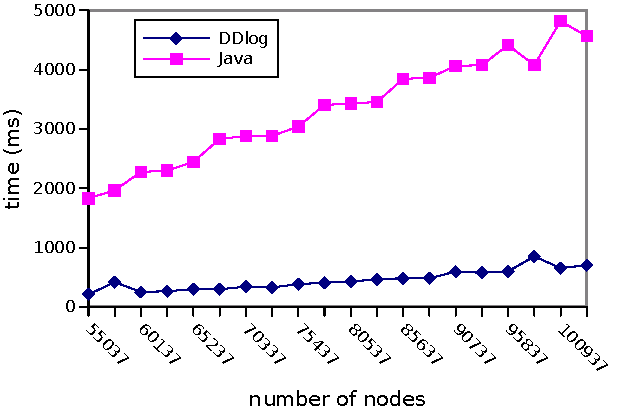
\includegraphics[width=.5\columnwidth]{non-incremental.pdf} &
      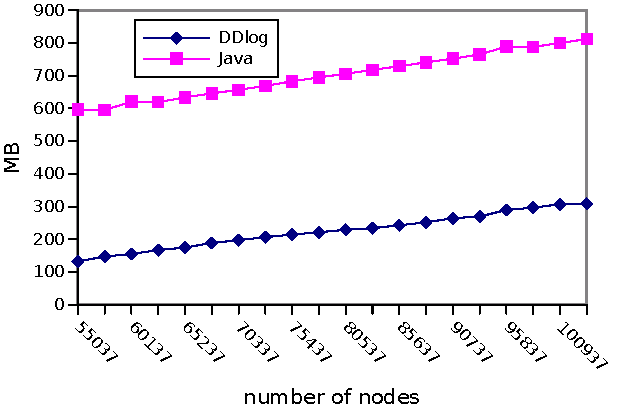
\includegraphics[width=.5\columnwidth]{memory.pdf} \\
      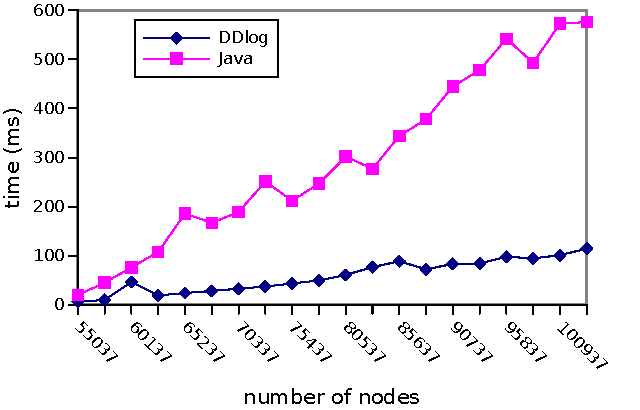
\includegraphics[width=.5\columnwidth]{insertion.pdf} &
      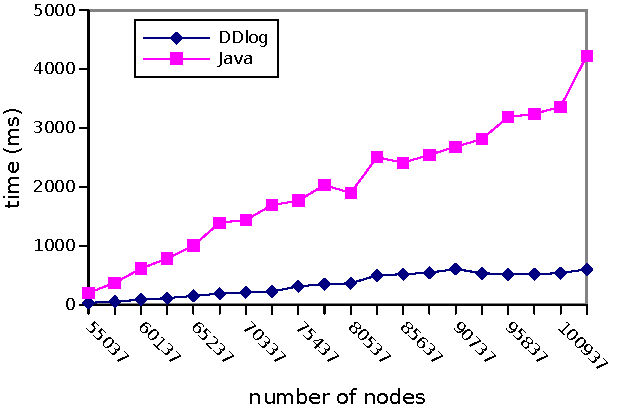
\includegraphics[width=.5\columnwidth]{deletion.pdf} \\
    \end{tabular}
  \end{center}
    \caption{DDlog performance.  (1) the time taken to execute the
      non-incremental reachability computation (inserting all nodes
      and edges in a single transaction); (2) the peak memory
      consumption; (3) the time to insert an additional 12\% edges
      into the graph for various graphs sizes, and (4) the time to
      delete 3\% of the edges.\label{fig:performance}}
\end{figure}
